\documentclass[../ClassicThesis.tex]{subfiles}
\begin{document}

%************************************************
\chapter{Userinteraction}\label{ch:userinteraction}
%************************************************

As our software is a converter, we minimized the required user interaction.

\section{Drag n Drop as Main Interaction}

Because the main function of our web service is converting custom objects, uploading a model is made easy by providing a drop area. This spread out over the whole web site.

\section{Customize View}

\subsection{Material Parameters}
\subsection{Device Parameters (Calibration)}

\section{Debug View}

\subsection{Pipeline Visualizations}
\subsection{Algorithm/ Method Selection}
\subsection{Testables (Operating Mode)}
\subsection{Console Debug Output}

\section{{\platener} as a Command Line Interface for Advanced Users}
\label{sec:walkthrough-cli}

We have seen in the preceding sections, how {\platener} is used in a
web browser.
% We intent to maximize scalability and user-friendliness
% by providing a web application.
Though converting a {\threedmodel} can be realized in a mere
drag-and-drop action using a web browser, we are limited to a single
conversion at a time. The web solution focuses on the results of the
conversion. Developers require a tool, that reports about the
conversion status and internal successful or failed processes. Our
software {\platener} provides a command line interface (CLI), which is
used in a terminal window. The CLI exposes commands for converting
{\threedmodel}s, processing multiple models in sequence and logging
progress reports. We explain the usage of the CLI in
Section~\sectionref{sec:walkthrough-cli-usage} and we demonstrate the logging
capabilities in Section~\sectionref{sec:walkthrough-cli-reports}.

\subsection{Usage Instructions of {\platener}'s CLI}
\label{sec:walkthrough-cli-usage}

A CLI is self-documenting. Listing~\ref{lst:cli-help} shows the
available commands.

\begin{listing}[!h]
\begin{minted}[
linenos
]{text}
node platener-cli.js -h

Specify an output directory.

  Usage: platener-cli [options] <output-dir>

  Options:

    -h, --help                output usage information
    -V, --version             output the version number
    -p --convertPath <input>  Convert multiple stl-Models to plates.
                              Give path to an folder with stl-Files.
    -f --convertFile <input>  Convert an stl-Model to plates.
                              Give path to an stl-File.
    -v --verbose              Enable Verbose Logging
    -s --subReports           Log Reports for each Fabrication Method
    --maxFilesize <input>     Limit filesize (MB),
                              so large files are skipped.

Full Help:

-f --convertFile    Generate all conversions for each
                    fabrication mode for the given stl-Model.
                    Each solution is stored in a seperate zip-File.
                    The zip-Files are written to the output directory.
\end{minted}
\caption{The help of {\platener}'s CLI.}
\label{lst:cli-help}
\end{listing}


The command line interface mirrors all the computational behavior of
{\platener} as a web application. With the CLI, we can convert a
single {\threedmodel} by loading data from the file system. The
conversion result is again a {\zipfile}. It is written to a given
target directory. We can recursively read input directories to
convert each {\stlfile} for the laser cutter. Both commands are given
in Listing~\ref{lst:cli-convert}.


\begin{listing}[!h]
\begin{minted}[
linenos
]{shell}
# convert a single file
node platener-cli.js -f ./stl/cubeFilled5cm.stl ./conversions

# convert an input directory
node platener-cli.js -f ./stl ./conversions
\end{minted}
\caption{Converting an {\stlfile} with {\platener}'s CLI.}
\label{lst:cli-convert}
\end{listing}

We can use the \emph{--maxFilesize} filter, to limit the
input files by their size in megabytes.

\subsection{Tracking Down Errors with Conversion Reports}
\label{sec:walkthrough-cli-reports}

Using the web application we either receive a successfully converted
{\svgfile} or the conversion fails. As the web interface is a
user-centered design we do not show extensive error messages or logs
of similar kind. For a developer it is crucial know where and under what
circumstances the software failed. With reports, we document the
conversion process. A report provides a short summary of the
conversion and gathers all error messages along the way, so a
developer can track down the issue. Figure~\ref{fig:report-simple}
shows a summary report. A report itemizing the results of our three
conversion approaches can be seen in Figure~\ref{fig:report-methods}.
In Figure~\ref{fig:report-error} an error message is depicted. When
multiple conversions were enqueued by {\platener}, we receive each
conversion report when the process finishes, as shown in
Figure~\ref{fig:report-multiple}.

\begin{figure}
  \centering
  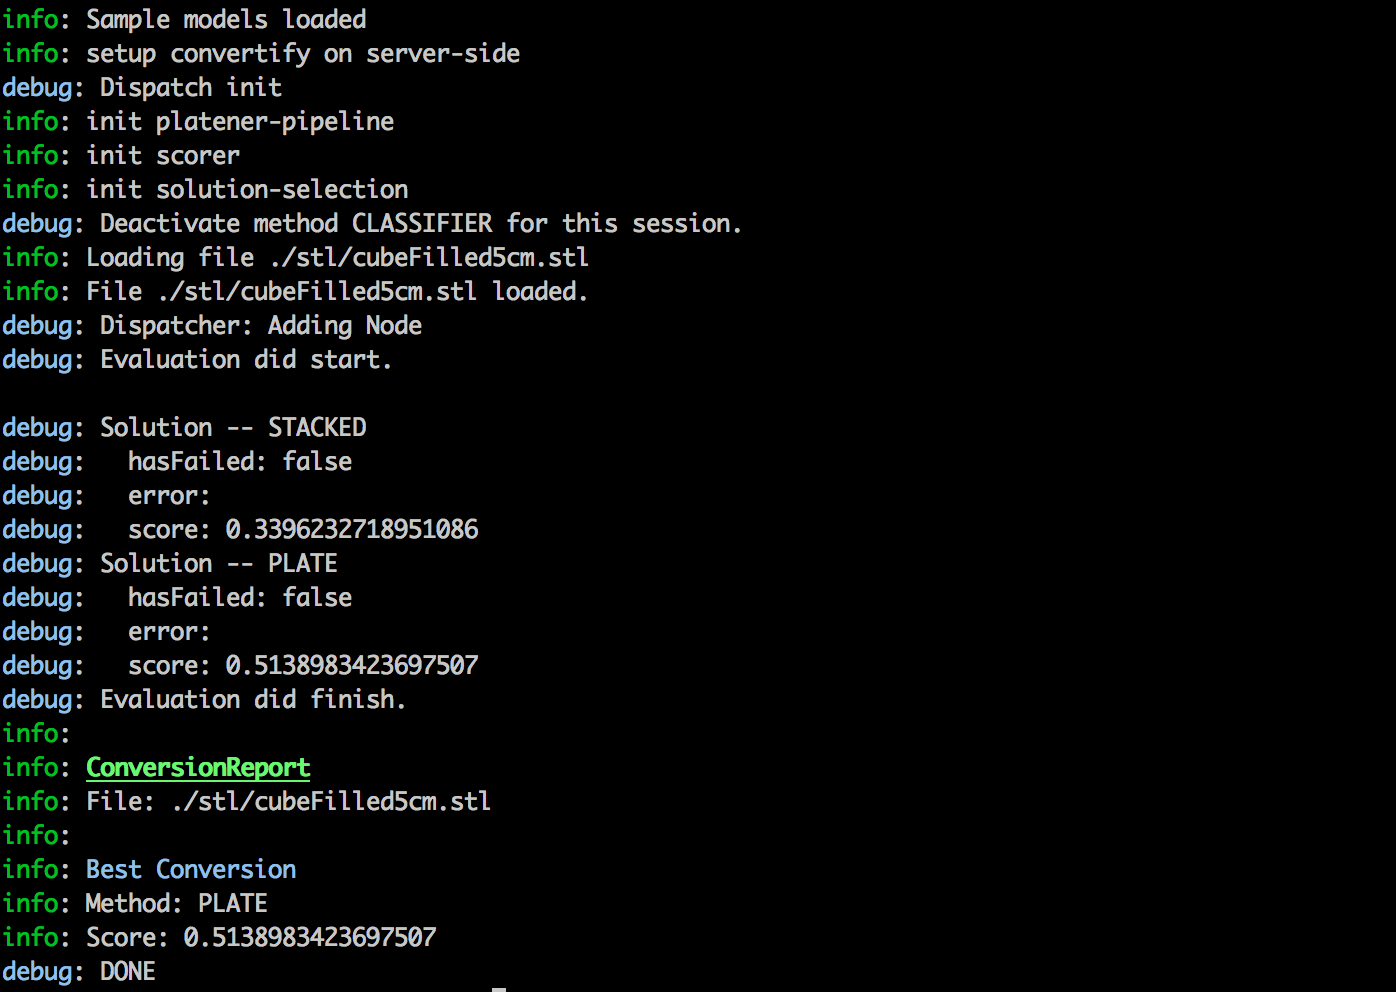
\includegraphics[width=1\columnwidth]{02-user-interaction-report-simple}
  \caption{A \class{Report}, showing a summary of the conversion.}
  \label{fig:report-simple}
\end{figure}

\begin{figure}
  \centering
  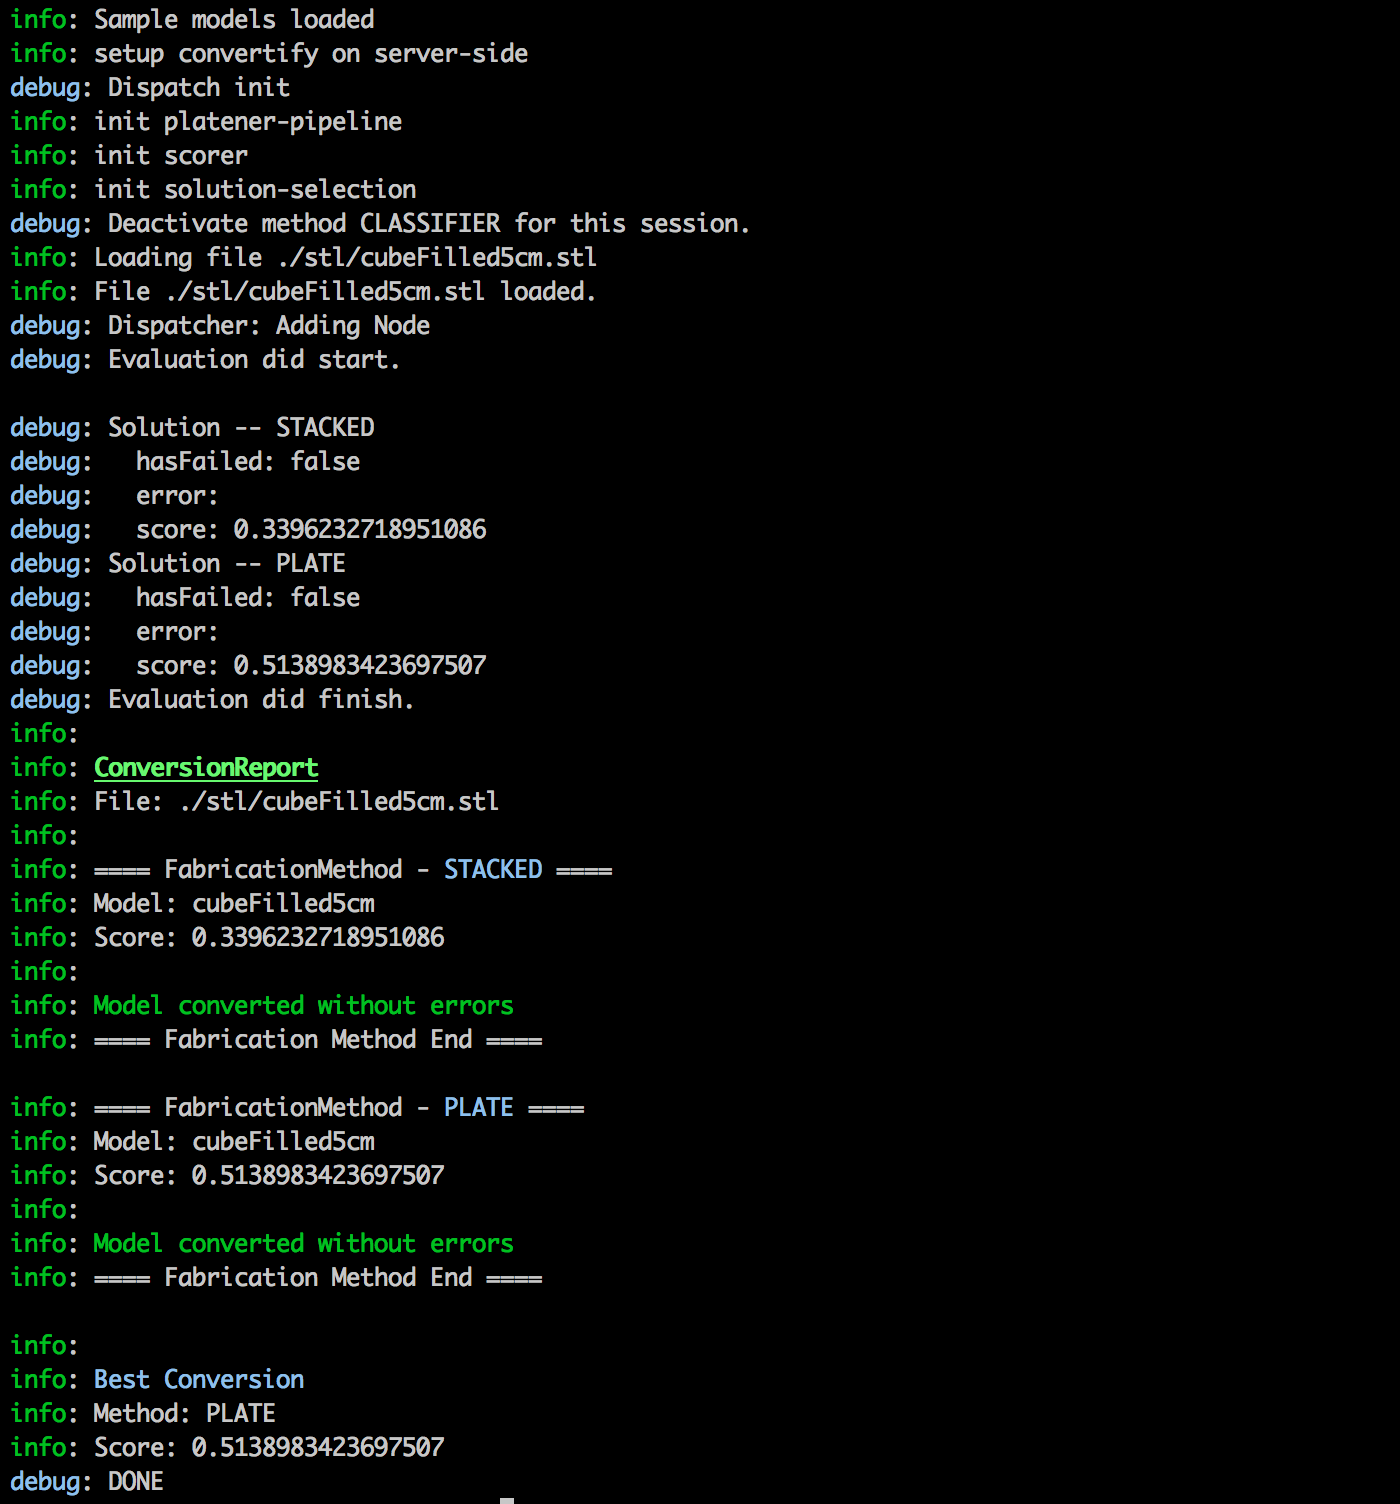
\includegraphics[width=1\columnwidth]{02-user-interaction-report-methods}
  \caption{A \class{Report}, showing a separate summary for each
    fabrication method of the conversion.}
  \label{fig:report-methods}
\end{figure}

\begin{figure}
  \centering
  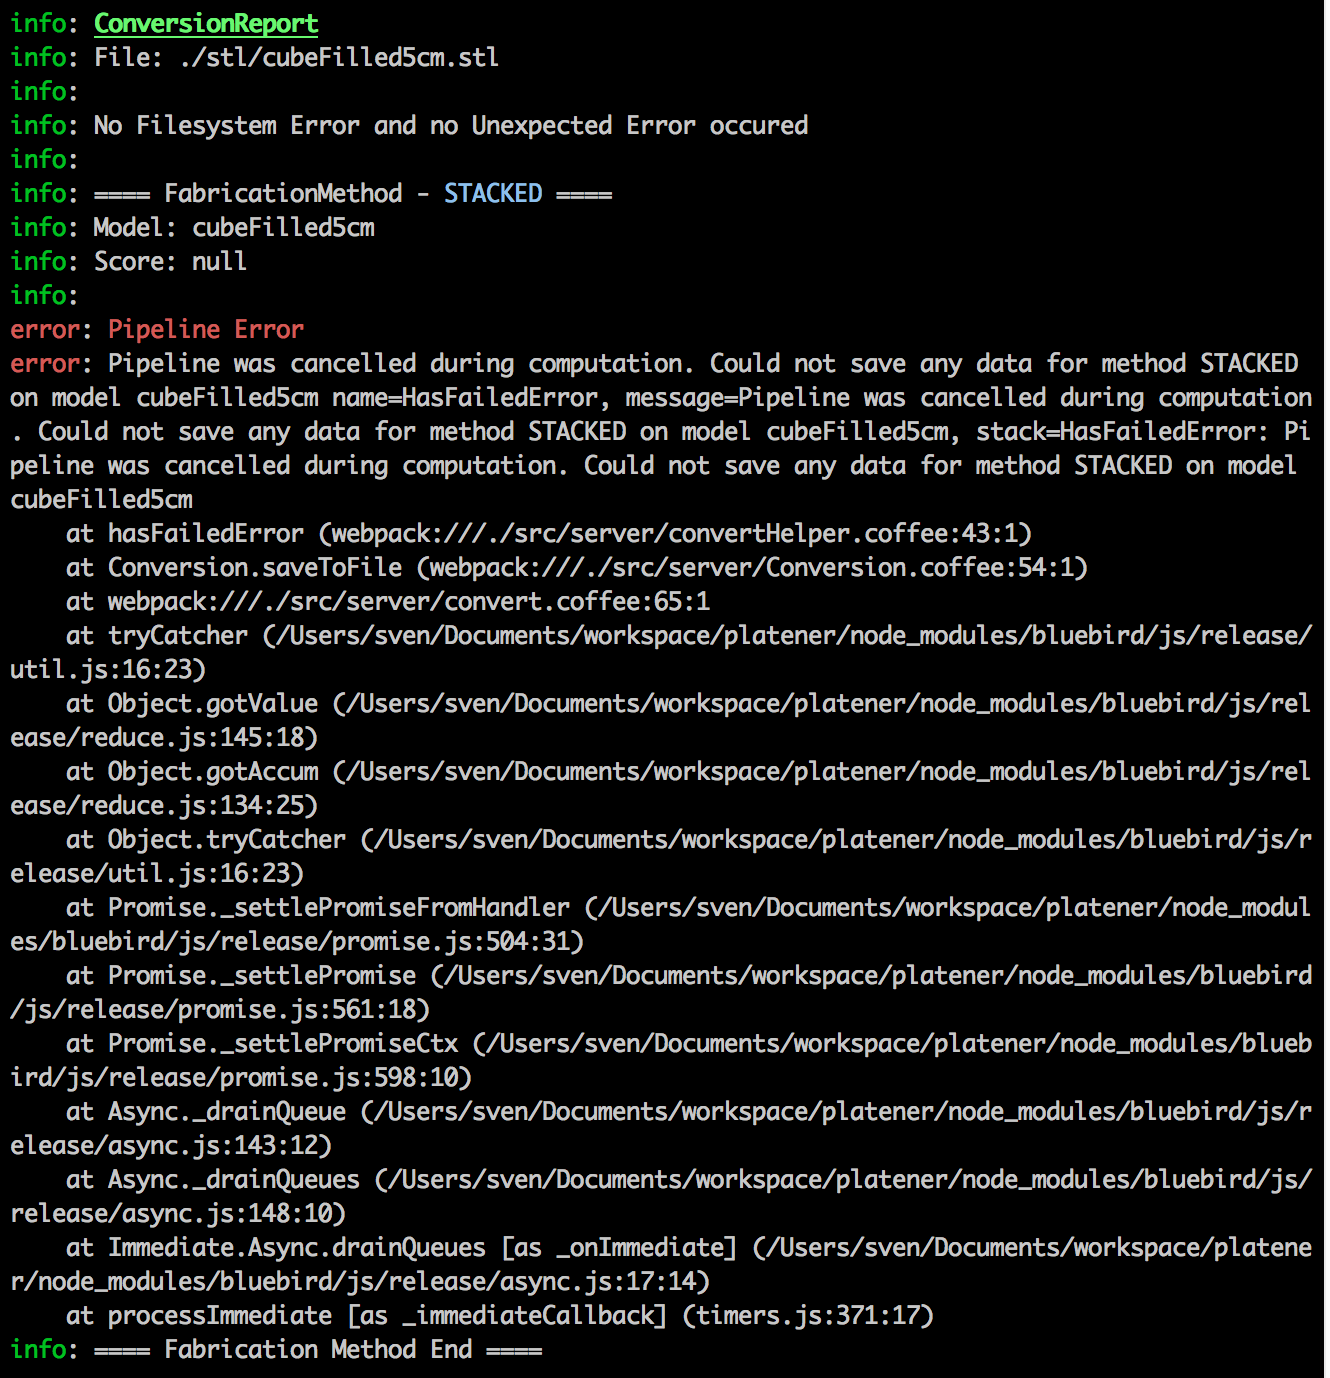
\includegraphics[width=0.8\columnwidth]{02-user-interaction-report-error}
  \caption{When a conversion fails the \class{Report} shows the error
    message.}
  \label{fig:report-error}
\end{figure}

\begin{figure}
  \centering
  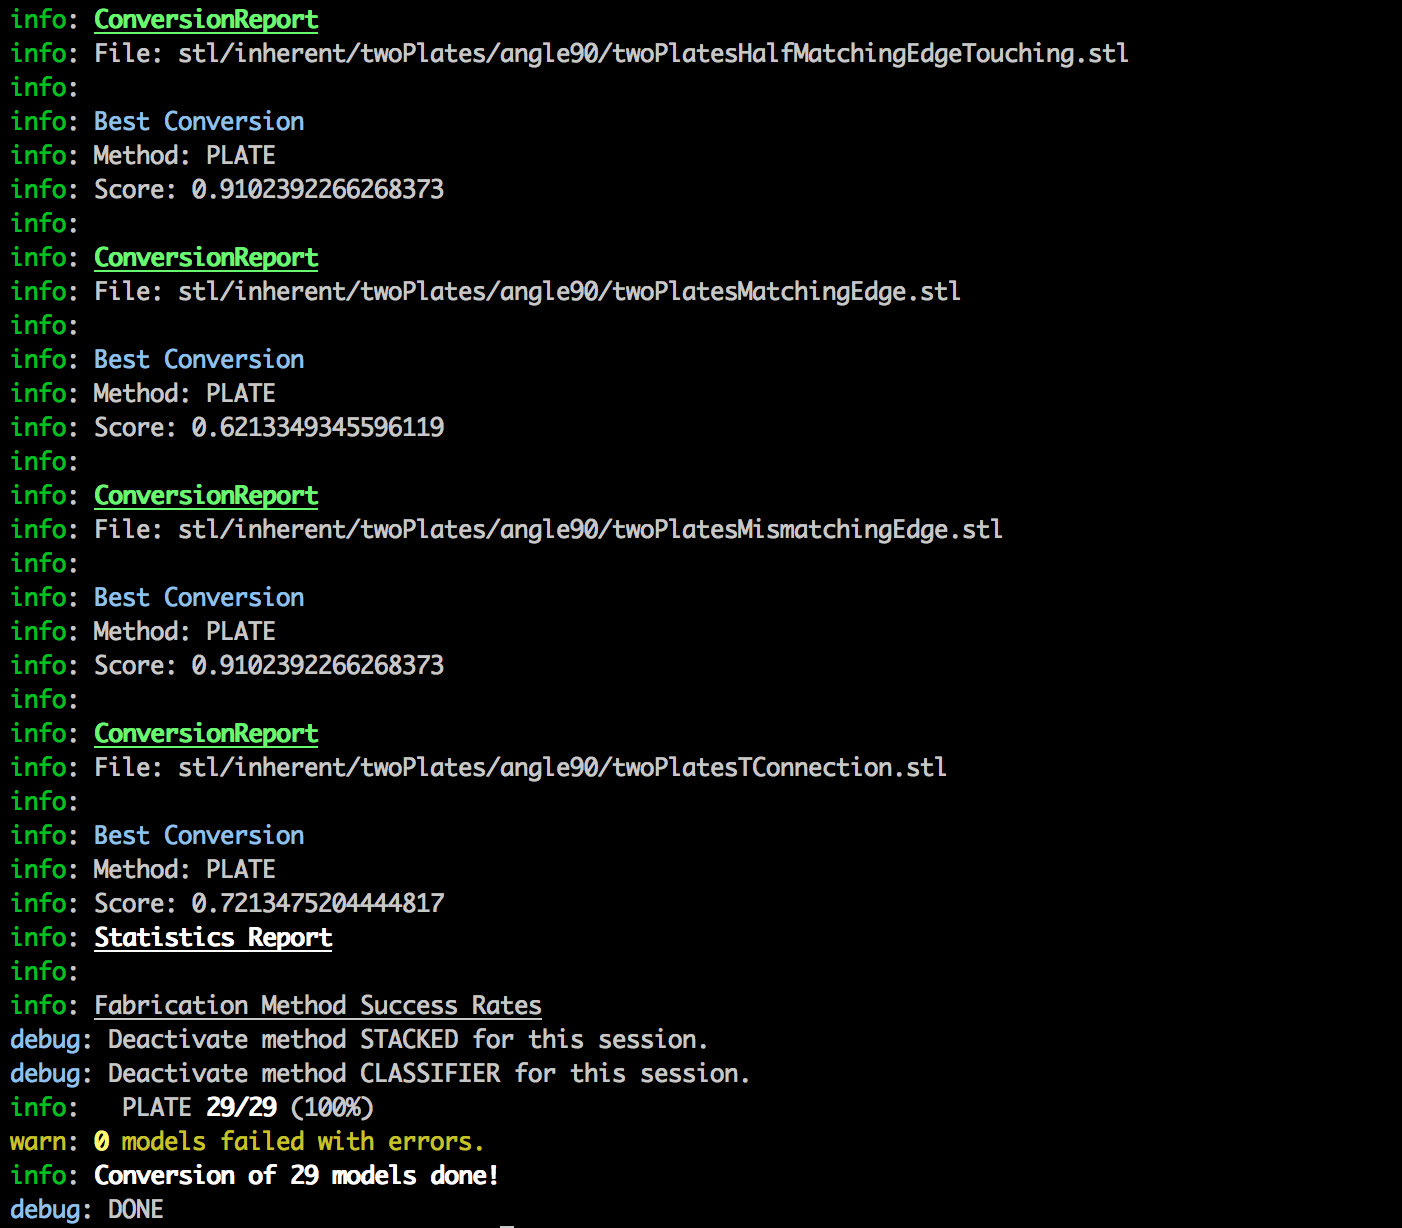
\includegraphics[width=0.8\columnwidth]{02-user-interaction-report-multiple}
  \caption{A sequence of conversions is summarized when the
    computation completed.}
  \label{fig:report-multiple}
\end{figure}



\end{document}

%%% Local Variables:
%%% mode: latex
%%% TeX-master: "../ClassicThesis"
%%% TeX-command-extra-options: "-shell-escape"
%%% End:
